% Generated by pysimcount.pffig13ext -- do not edit; regenerate instead.
% figure: fig13ext-cnot-lines-after -- Fig. 13 extended, CNOT, without Lie-Trotter S1, Suzuki S2, Suzuki S8; after optimisation only (circles)
% metric=cnot gatebase=cz unmerged; r_method=measured-fit: r = ceil(a n^b) fitted to measured r, mean over seeds [1, 2, 3, 4, 5, 6, 7, 8, 9, 10], n = [5, 6, 7, 8, 9, 10, 11]; every point extrapolated; y axis autoscaled (not the replica's range)
% optimised = Light reconstruction r x marginal + edge; verified n <= 16
% figure made at git_commit=3f419fd078cbd27a6e57919468bd4e5f1b96c08b git_dirty=False
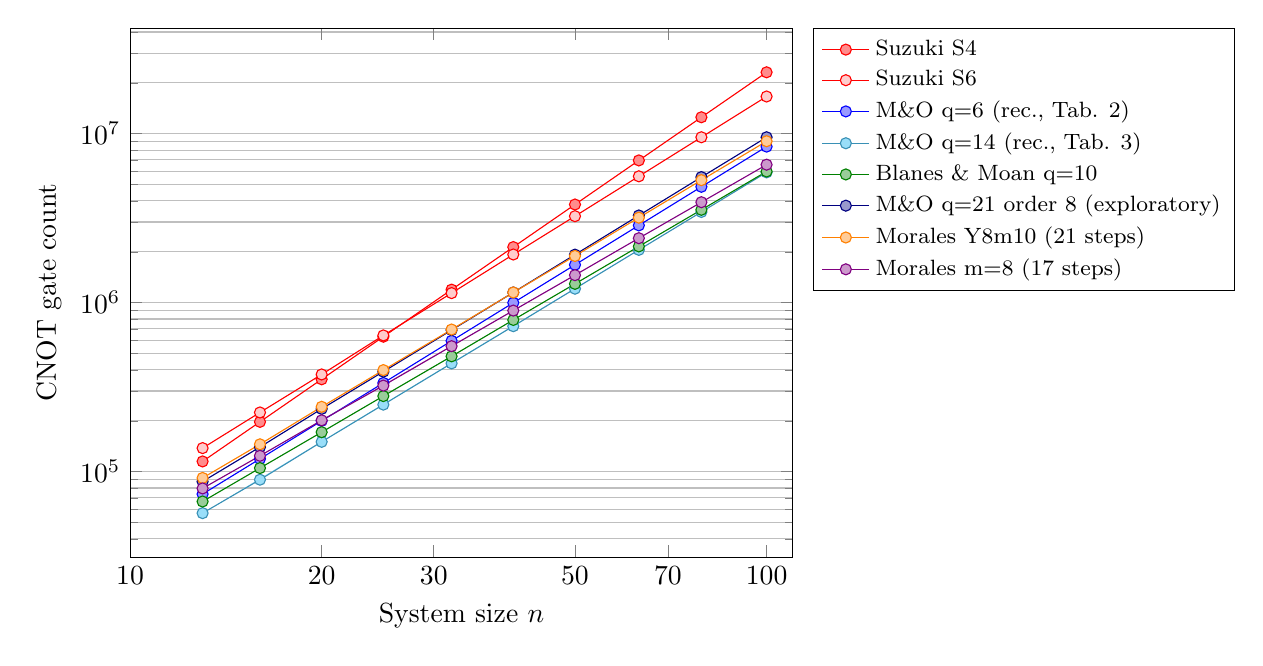
\begin{tikzpicture}
  \begin{loglogaxis}[
    width=10cm, height=8.3cm,
    xlabel={System size $n$}, ylabel={CNOT gate count},
    xmin=10, xmax=110,
    xtick={10,20,30,50,70,100}, xticklabels={10,20,30,50,70,100},
    ymajorgrids=true, yminorgrids=true,
    legend pos=outer north east, legend cell align=left,
    legend style={font=\footnotesize},
  ]
    \addplot[solid, mark=*, mark size=2pt, draw=red, fill=red!45] coordinates {
      (13,114946)
      (16,197152)
      (20,352040)
      (25,629050)
      (32,1194304)
      (40,2132880)
      (50,3810100)
      (63,6947766)
      (79,12510598)
      (100,23084200)
    };
    \addlegendentry{Suzuki S4}
    \addplot[solid, mark=*, mark size=2pt, draw=red, fill=red!20] coordinates {
      (13,137826)
      (16,224032)
      (20,376040)
      (25,640050)
      (32,1139264)
      (40,1928080)
      (50,3250100)
      (63,5594526)
      (79,9527558)
      (100,16600200)
    };
    \addlegendentry{Suzuki S6}
    \addplot[solid, mark=*, mark size=2pt, draw=blue, fill=blue!40] coordinates {
      (13,73658)
      (16,119072)
      (20,199720)
      (25,334850)
      (32,594496)
      (40,998480)
      (50,1675300)
      (63,2866878)
      (79,4850126)
      (100,8385800)
    };
    \addlegendentry{M\&O q=6 (rec., Tab. 2)}
    \addplot[solid, mark=*, mark size=2pt, draw=cyan!70!black, fill=cyan!40] coordinates {
      (13,56810)
      (16,89632)
      (20,150120)
      (25,249250)
      (32,437312)
      (40,725840)
      (50,1209700)
      (63,2053422)
      (79,3442030)
      (100,5902600)
    };
    \addlegendentry{M\&O q=14 (rec., Tab. 3)}
    \addplot[solid, mark=*, mark size=2pt, draw=green!50!black, fill=green!50!black!40] coordinates {
      (13,66586)
      (16,104992)
      (20,171240)
      (25,280050)
      (32,481344)
      (40,790480)
      (50,1292100)
      (63,2152206)
      (79,3545678)
      (100,5976200)
    };
    \addlegendentry{Blanes \& Moan q=10}
    \addplot[solid, mark=*, mark size=2pt, draw=blue!50!black, fill=blue!50!black!40] coordinates {
      (13,87386)
      (16,139808)
      (20,235240)
      (25,390650)
      (32,688192)
      (40,1149200)
      (50,1923700)
      (63,3281166)
      (79,5534582)
      (100,9525800)
    };
    \addlegendentry{M\&O q=21 order 8 (exploratory)}
    \addplot[solid, mark=*, mark size=2pt, draw=orange, fill=orange!40] coordinates {
      (13,91754)
      (16,145184)
      (20,241960)
      (25,399050)
      (32,693568)
      (40,1149200)
      (50,1890100)
      (63,3185910)
      (79,5308958)
      (100,9021800)
    };
    \addlegendentry{Morales Y8m10 (21 steps)}
    \addplot[solid, mark=*, mark size=2pt, draw=violet, fill=violet!40] coordinates {
      (13,79586)
      (16,124064)
      (20,201320)
      (25,323050)
      (32,552768)
      (40,897680)
      (50,1455300)
      (63,2407734)
      (79,3932462)
      (100,6555400)
    };
    \addlegendentry{Morales m=8 (17 steps)}
  \end{loglogaxis}
\end{tikzpicture}
